% This is A English TeX Template for Thesis to be submitted to Zhejiang University for Bachelor's Degree.
% This template is licensed under the GNU General Public License, version 2 (GPL v2), which can be obtained at http://www.gnu.org/licenses/gpl-2.0.html
% The format generally accords with the formatting requirement of ZJU Dept Mat Sci Eng. For a complete list of changes please refer to the ReadMe file.
% Part of the formatting codes are modified from naoz's template for College of EE.

% To Start, compile with XeLaTex in order to handle UTF characters (chinese)

\documentclass[a4paper,twoside,12pt]{book}
\usepackage{indentfirst}
\usepackage{graphicx}
\usepackage{fancyhdr}
\usepackage[top=2.54cm,bottom=2.54cm,left=3.17cm,right=3.17cm]{geometry}
\usepackage{setspace}
\usepackage{titlesec}
\usepackage{titletoc}
\usepackage{fontspec}
\usepackage{hyperref}
\usepackage{cleveref}
%\usepackage{achemso}
\usepackage[square,numbers,super,sort&compress]{natbib}
\usepackage{mhchem}
\usepackage{pdfpages}
\usepackage{gensymb}
\usepackage{xspace}
\usepackage[labelsep=space,font=small,labelfont=bf]{caption}

% Font family and size; Chinese bold
% Works on Windows with TeX Live (MikTeX)
% Check fonts installation and license first
\newcommand{\song}{\fontspec{SimSun}\selectfont}
\newcommand{\songb}{\fontspec{SimSun:embolden=4}\selectfont}
\newcommand{\fs}{\fontspec{FangSong}\selectfont}
\newcommand{\fsb}{\fontspec{FangSong:embolden=4}\selectfont}
\newcommand{\tnr}{\fontspec{Times New Roman}\selectfont}
\setmainfont{Times New Roman}

\newcommand{\chuhao}{\fontsize{42pt}{\baselineskip}\selectfont}
\newcommand{\xiaochu}{\fontsize{36pt}{\baselineskip}\selectfont}
\newcommand{\yihao}{\fontsize{26pt}{\baselineskip}\selectfont}
\newcommand{\xiaoyi}{\fontsize{24pt}{\baselineskip}\selectfont}
\newcommand{\erhao}{\fontsize{22pt}{\baselineskip}\selectfont}
\newcommand{\xiaoer}{\fontsize{18pt}{\baselineskip}\selectfont}
\newcommand{\sanhao}{\fontsize{16pt}{\baselineskip}\selectfont}
\newcommand{\xiaosan}{\fontsize{15pt}{\baselineskip}\selectfont}
\newcommand{\sihao}{\fontsize{14pt}{\baselineskip}\selectfont}
\newcommand{\xiaosi}{\fontsize{12pt}{\baselineskip}\selectfont}
\newcommand{\wuhao}{\fontsize{10.5pt}{\baselineskip}\selectfont}
\newcommand{\xiaowu}{\fontsize{9pt}{\baselineskip}\selectfont}
\newcommand{\liuhao}{\fontsize{7.5pt}{\baselineskip}\selectfont}
\newcommand{\xiaoliu}{\fontsize{6.5pt}{\baselineskip}\selectfont}
\newcommand{\qihao}{\fontsize{5.5pt}{\baselineskip}\selectfont}
\newcommand{\bahao}{\fontsize{5pt}{\baselineskip}\selectfont}

\onehalfspace

% Latin words
\newcommand{\etal}{\textit{et al.}\xspace}
\newcommand{\ie}{\textit{i.e.}\xspace}
\newcommand{\eg}{\textit{e.g.}\xspace}
\newcommand{\ca}{\textit{ca.}\xspace}
\newcommand{\insitu}{\textit{in-situ}\xspace}

\newcommand\reaction[1]{\begin{equation}\ce{#1}\end{equation}}
\renewcommand*{\thefootnote}{\fnsymbol{footnote}}

% chapter title rules
\makeatletter
\renewcommand\chapter{\if@openright\cleardoublepage\else\clearpage\fi
	%\thispagestyle{empty}% original style: plain
	\global\@topnum\z@
	\@afterindentfalse
	\secdef\@chapter\@schapter}
\makeatother

% blank page rules
\makeatletter
\def\cleardoublepage{\clearpage%
	\if@twoside
	\ifodd\c@page\else
	\vspace*{\fill}
	\hfill
	\begin{center}
		[This page intentionally left blank]
	\end{center}
	\vspace{\fill}
%	\thispagestyle{empty}
	\newpage
	\if@twocolumn\hbox{}\newpage\fi
	\fi
	\fi
}
\makeatother


\begin{document}
	%==================================================
	%                   Settings
	%==================================================
	% page styles
	\fancypagestyle{main}{ %
		\fancyhf{}
		\renewcommand{\headrulewidth}{0.5pt}
		\fancyhead[EC]{\xiaowu\fontspec{SimSun}\selectfont{浙江大学学士学位论文}}
		\fancyhead[OC]{\xiaowu \leftmark}
		\fancyfoot[OR]{\xiaowu\arabic{page}}
		\fancyfoot[EL]{\xiaowu\arabic{page}}
		}
	
	% Make subscript in equations in regular type rather than italic, enable if needed 
	% \let\sb=_ \catcode`\_=\active \def_#1{\ensuremath \sb{\rm#1}}
	
	% Change the label of Figures and Tables, enable if needed (e.g., change to Chinese)
%	\renewcommand{\thefigure}{\textbf{\thechapter.\arabic{figure}}} 
%	\renewcommand{\figurename}{\textbf{Figure}}
%	\renewcommand{\thetable}{\textbf{\thesection.\arabic{table}}} 
%	\renewcommand{\tablename}{\textbf{Table}}
	
	% Headings
	\titleformat{\chapter}%
	  {\center\Large\bfseries\sanhao}{Chapter \thechapter}{1em}{}{}
	\titlespacing{\chapter}%
	  {0pt}{0pt}{18pt}
	\titlecontents{chapter}[0em]{}%
	{Chapter \thecontentslabel.\quad}{\hspace{0em}}{\titlerule*[10pt]{.}\contentspage}
	
	\titleformat{\section}[hang]%
	{\large\bfseries\sihao}{\thesection}{1em}{}{}
	\titlespacing{\section}%
	  {0pt}{24pt}{6pt}
	\titlecontents{section}[4.0em]{}%
	  {\contentslabel{2.0em}}{\hspace{3em}}{\titlerule*[10pt]{.}\contentspage}
	
	\titleformat{\subsection}[hang]%
	  {\sihao\bfseries\xiaosi}{\thesubsection}{1em}{}{}
	\titlespacing{\subsection}%
	  {0pt}{12pt}{6pt}
	\titlecontents{subsection}[8.0em]{}%
	  {\contentslabel{4.0em}}{\hspace{3em}}{\titlerule*[10pt]{.}\contentspage}
	
	
	
	%==================================================
	%            Title, abstract and contents
	%==================================================
	%==Title==
	\begin{titlepage}
	\begin{center}
		\large \doublespacing
		An Amazing English Dissertation Template Which Will Impress Your Committee \\[3em]	
		
		By\\		
		Jingshan Du \\[3em]
		
		A thesis submitted in partial satisfaction\\ of the requirement for\\		
		Bachelor's Degree\\		
		in\\		
		Engineering: Materials Science and Engineering\\		
		in\\		
		Zhejiang University \\[3em]
		
		Supervised by
		
		Professor Awesome Advisor\\[6em]
		
		Summer 2015
		\newpage
		\thispagestyle{empty}
		\null\vfill
		\texttt{\copyright~2015 by Jingshan Du\\All rights reserved.}
	\end{center}
	
\end{titlepage}
		
	\pagestyle{main}
	\fancyfoot[OR]{\xiaowu\Roman{page}} 
	\fancyfoot[EL]{\xiaowu\Roman{page}} 
	\setcounter{page}{1}
	
	%==Abstract==
	\chapter*{Abstract\markboth{ABSTRACT}{}}
	\fontsize{12pt}{20pt}
	This is the place where you want to put your abstract. Note that you should choose several keywords as below as required by your department.


\hangafter=1
\setlength{\hangindent}{6.5em}
\textbf{Keywords: }first, second, more, even more
	
	%==Abstract CN==
	\chapter*{\fsb 摘~要\markboth{\xiaowu \song 摘~要}{}}
	\fontsize{12pt}{20pt}
	{
	\fs \XeTeXlinebreaklocale "zh" \XeTeXlinebreakskip = 0pt plus 1pt minus 0.1pt
	\parindent 2em
	中文摘要在这里。注意由于中英文混排的时候,XeLaTeX 对中文字符的排版格式例如 hanging 好像不能正常支持,所以下方关键词的换行用了一个hack……


{\fsb 关键词:}第一个,第二个,第三个,第四个,还有吗,

~~~~~~~~还有一个 % this is a hack...
	}
	\cleardoublepage
	
	%==TOC==
	\pagestyle{empty}
	\tableofcontents
	\listoffigures
	%\listoftables
	\cleardoublepage

	
	
	%==================================================
	%                   Main Body
	%==================================================
	\pagestyle{main}

	\setcounter{page}{1}
	\chapter{Introduction}
\section{Already main text??!}

But it isn't too fast right? Let's see how graphics work. Don't forget to use\\ \verb|\caption[in Table of Figure]{in body}| and\\ \verb|\label{referable lable for you}|.

\begin{figure}
	\centering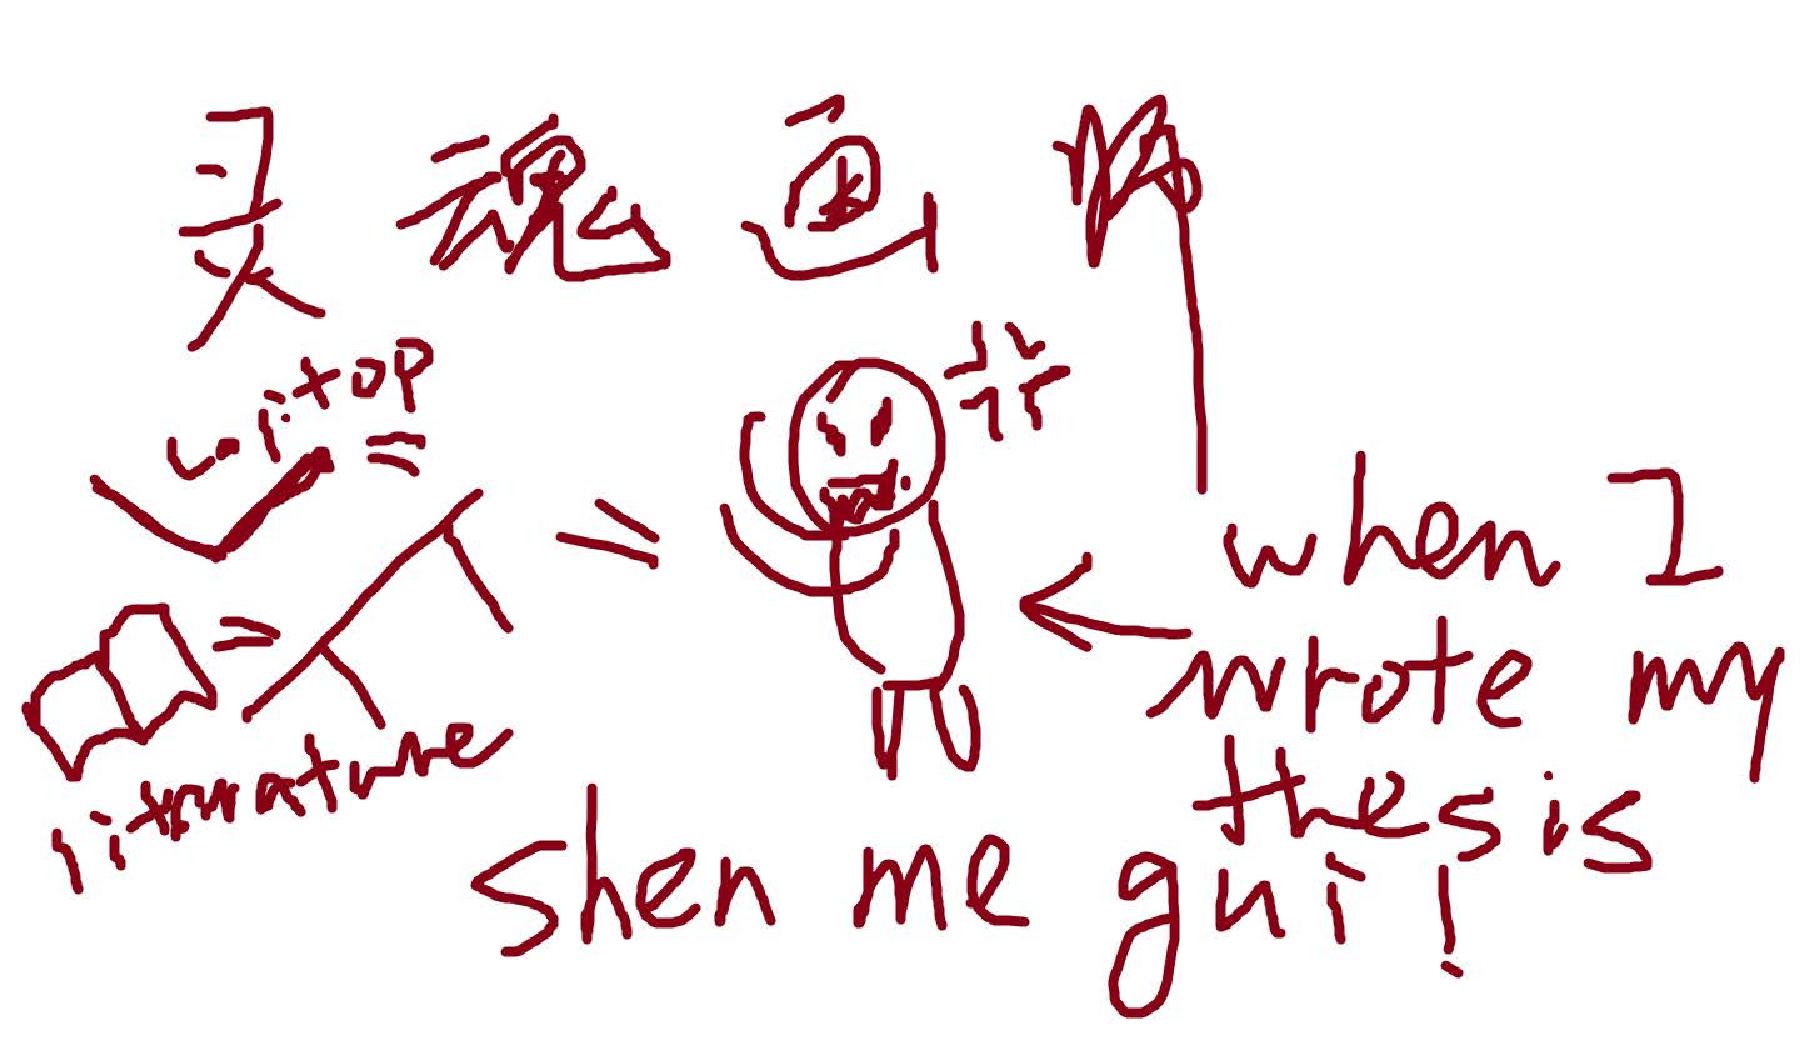
\includegraphics[width=0.7\textwidth]{figure/1-TOC.pdf}
	\caption[Schematic illustration of how I feel when writing my thesis]{Schematic illustration of how I feel when writing my thesis and showing my outstanding drawing technique.}\label{fig1-TOC}
\end{figure}

Look, according to \autoref{fig1-TOC} am I good at drawing? This is evidenced by a literature!\cite{mywork}

This dissertation is reproduced with permission in part from an unpublished manuscript: 
\begin{quote}
	Me Obviously, Good Partner, Someone Else, My Boss. Super Really Very Cool Paper To Be Published. \textbf{2015}.
\end{quote} 

This dissertation is accompanied by three supporting movies (Movie S1-S3), which are available upon request to \href{mailto:dujingshan@zju.edu.cn}{dujingshan@zju.edu.cn}. P.S. Of course not in this template. :P


	%==References==
	\cleardoublepage
	\phantomsection
	\renewcommand{\bibname}{References}
	\addcontentsline{toc}{chapter}{References}
	
	% Install if needed: https://github.com/Haixing-Hu/GBT7714-2005-BibTeX-Style
	\bibliographystyle{gbt7714-2005}
	\setlength\bibsep{0pt}
	\bibliography{bib/ref}
	
	\cleardoublepage
	
		%==Acknowledgements==
		\chapter*{Acknowledgments\markboth{ACKNOWLEDGMENTS}{}}
		\addcontentsline{toc}{chapter}{Acknowledgments}
		You definitely want to acknowledge a lot of people. Write here to express~
		\cleardoublepage
\end{document}